\documentclass[preview]{standalone}
\usepackage{tikz}
\usepackage{amsmath}
\usepackage{xcolor}
\usetikzlibrary{arrows.meta, decorations.pathmorphing}

\begin{document}
\begin{frame}{\textbf{From Band Structure to Correlations}}
\begin{center}
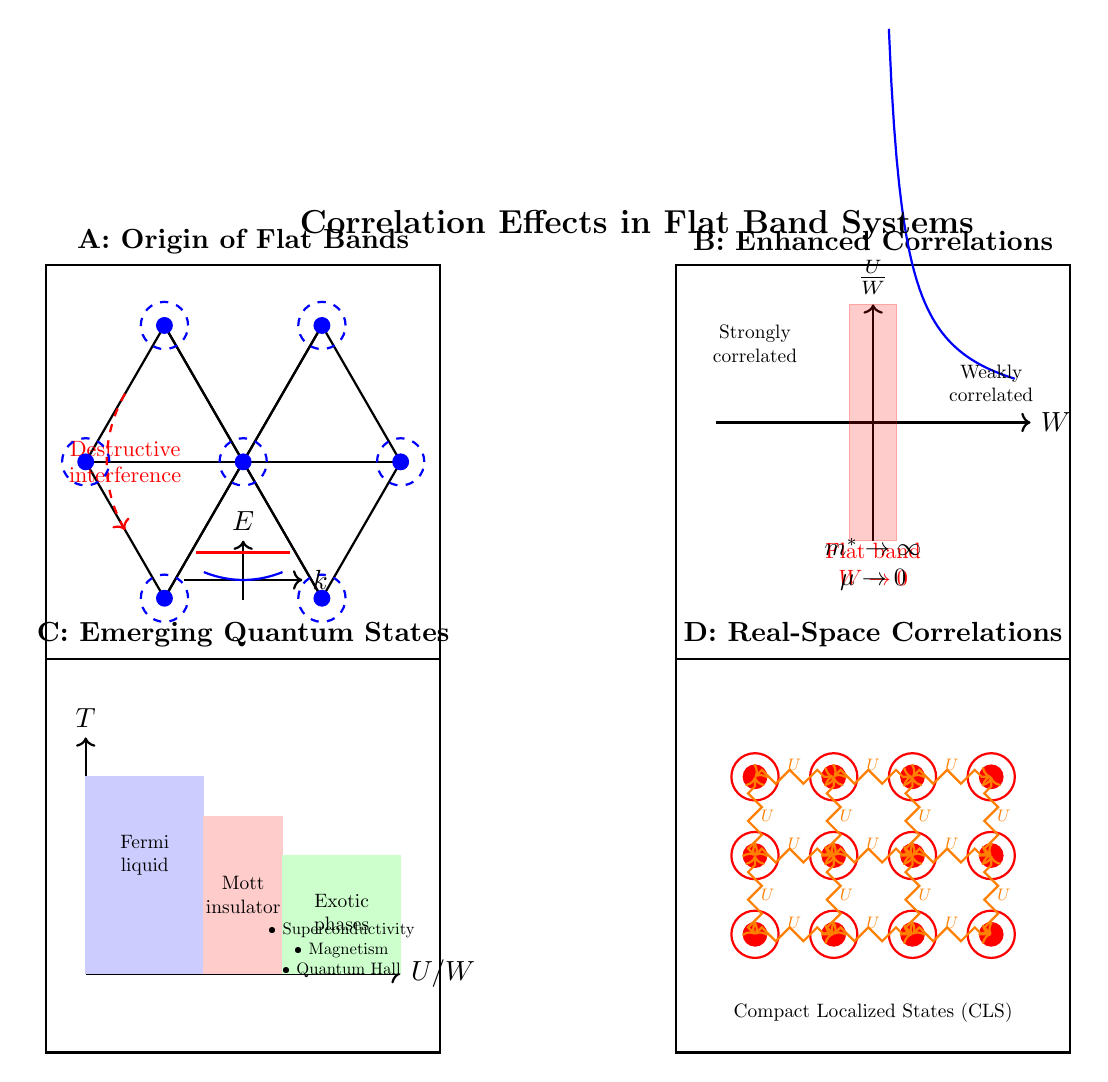
\begin{tikzpicture}[scale=1.0]
    % PANEL A: ORIGIN OF FLAT BANDS
    \begin{scope}[shift={(-5,3)}]
        \draw[thick] (-2.5,-2.5) rectangle (2.5,2.5);
        \node at (0,2.8) {\textbf{A: Origin of Flat Bands}};
        
        % Kagome lattice (simplified)
        \draw[thick] (-2,0) -- (0,0) -- (2,0);
        \draw[thick] (-1,1.732) -- (0,0) -- (1,1.732);
        \draw[thick] (-1,-1.732) -- (0,0) -- (1,-1.732);
        \draw[thick] (-2,0) -- (-1,1.732) -- (0,0) -- (-1,-1.732) -- (-2,0);
        \draw[thick] (2,0) -- (1,1.732) -- (0,0) -- (1,-1.732) -- (2,0);
        
        % Destructive interference annotation
        \draw[->, dashed, thick, red] (-1.5,0.866) arc (150:210:1.732);
        \node[red, align=center, scale=0.8] at (-1.5,0) {Destructive\\interference};
        
        % Wave functions
        \foreach \x/\y in {-2/0, 0/0, 2/0, -1/1.732, 1/1.732, -1/-1.732, 1/-1.732} {
            \filldraw[blue] (\x,\y) circle (0.1);
            \draw[blue, thick, dashed] (\x,\y) circle (0.3);
        }
        
        % Resulting band structure
        \begin{scope}[shift={(0,-1.5)}, scale=0.5]
            \draw[->, thick] (-1.5,0) -- (1.5,0) node[right] {$k$};
            \draw[->, thick] (0,-0.5) -- (0,1) node[above] {$E$};
            \draw[thick, red] (-1.2,0.7) -- (1.2,0.7);
            \draw[thick, blue] plot[domain=-1:1, samples=20] (\x,{0.2*\x*\x});
        \end{scope}
    \end{scope}
    
    % PANEL B: CORRELATION ENHANCEMENT
    \begin{scope}[shift={(3,3)}]
        \draw[thick] (-2.5,-2.5) rectangle (2.5,2.5);
        \node at (0,2.8) {\textbf{B: Enhanced Correlations}};
        
        % U/W diagram
        \begin{scope}[shift={(0,0.5)}]
            \draw[->, thick] (-2,0) -- (2,0) node[right] {$W$};
            \draw[->, thick] (0,-1.5) -- (0,1.5) node[above] {$\frac{U}{W}$};
            
            % U/W curve
            \draw[thick, blue, domain=0.2:1.8, samples=50] 
                plot (\x,{1/\x});
            
            % Annotations
            \node[align=center, scale=0.7] at (1.5,0.5) {Weakly\\correlated};
            \node[align=center, scale=0.7] at (-1.5,1) {Strongly\\correlated};
            
            % Flat band regime
            \filldraw[red, opacity=0.2] (-0.3,-1.5) rectangle (0.3,1.5);
            \node[red, align=center, scale=0.8] at (0,-1.8) {Flat band\\$W \rightarrow 0$};
        \end{scope}
        
        % Effective mass and mobility
        \begin{scope}[shift={(0,-1.5)}, scale=0.6]
            \node[align=center, scale=0.9] at (0,0.7) {$m^* \rightarrow \infty$};
            \node[align=center, scale=0.9] at (0,0) {$\mu \rightarrow 0$};
        \end{scope}
    \end{scope}
    
    % PANEL C: EMERGING PHASES
    \begin{scope}[shift={(-5,-2)}]
        \draw[thick] (-2.5,-2.5) rectangle (2.5,2.5);
        \node at (0,2.8) {\textbf{C: Emerging Quantum States}};
        
        % Phase diagram
        \draw[->, thick] (-2,-1.5) -- (2,-1.5) node[right] {$U/W$};
        \draw[->, thick] (-2,-1.5) -- (-2,1.5) node[above] {$T$};
        
        % Phases
        \filldraw[blue!20] (-2,-1.5) rectangle (-0.5,1);
        \filldraw[red!20] (-0.5,-1.5) rectangle (0.5,0.5);
        \filldraw[green!20] (0.5,-1.5) rectangle (2,0);
        
        % Labels
        \node[align=center, scale=0.7] at (-1.25,0) {Fermi\\liquid};
        \node[align=center, scale=0.7] at (0,-0.5) {Mott\\insulator};
        \node[align=center, scale=0.7] at (1.25,-0.75) {Exotic\\phases};
        
        % Sub-phases
        \node[align=center, scale=0.6] at (1.25,-1.2) {• Superconductivity\\• Magnetism\\• Quantum Hall};
    \end{scope}
    
    % PANEL D: REAL-SPACE CORRELATIONS
    \begin{scope}[shift={(3,-2)}]
        \draw[thick] (-2.5,-2.5) rectangle (2.5,2.5);
        \node at (0,2.8) {\textbf{D: Real-Space Correlations}};
        
        % Localized electrons
        \foreach \x/\y in {-1.5/-1, -0.5/-1, 0.5/-1, 1.5/-1, 
                           -1.5/0, -0.5/0, 0.5/0, 1.5/0,
                           -1.5/1, -0.5/1, 0.5/1, 1.5/1} {
            \filldraw[red] (\x,\y) circle (0.15);
            \draw[red, thick] (\x,\y) circle (0.3);
        }
        
        % Interaction lines
        \foreach \x/\y in {-1.5/-1, -0.5/-1, 0.5/-1, 
                          -1.5/0, -0.5/0, 0.5/0,
                          -1.5/1, -0.5/1, 0.5/1} {
            \draw[<->, orange, thick, decoration={zigzag}, decorate]
                (\x,\y) -- ({\x+1},\y) node[midway, above, orange, scale=0.6] {$U$};
        }
        
        \foreach \x/\y in {-1.5/-1, -0.5/-1, 0.5/-1, 1.5/-1,
                          -1.5/0, -0.5/0, 0.5/0, 1.5/0} {
            \draw[<->, orange, thick, decoration={zigzag}, decorate]
                (\x,\y) -- (\x,{\y+1}) node[midway, right, orange, scale=0.6] {$U$};
        }
        
        % Annotation
        \node[align=center, scale=0.7] at (0,-2) {Compact Localized States (CLS)};
    \end{scope}
    
    % MAIN TITLE
    \node[align=center, font=\large\bfseries] at (0,6) {Correlation Effects in Flat Band Systems};
\end{tikzpicture}

\end{center}
\end{frame}
\end{document}
